\documentclass[11pt,a4paper]{article}
\usepackage[margin=25mm]{geometry}
\usepackage{amsmath,amssymb,booktabs,graphicx,fancyhdr,hyperref,float}
\usepackage[T1]{fontenc}
\hypersetup{colorlinks=true,linkcolor=blue,urlcolor=blue,citecolor=blue}
\pagestyle{fancy}\fancyhf{}\fancyhead[C]{TEAM NUMBER REQUIRED}\fancyfoot[C]{\thepage}
\setlength{\headheight}{15pt}\setlength{\parskip}{3pt}\setlength{\parindent}{0pt}
\usepackage{caption}
\captionsetup{font=small,labelfont=bf}
\graphicspath{{../../img/}}
\begin{document}
\begin{center}
{\large Team: TEAM NUMBER REQUIRED}\par\vspace{12mm}
{\Large Problem B}\par\vspace{10mm}
{\LARGE Predicting a Penalty Kick from 0.10 Seconds of Motion}\par\vspace{8mm}
\end{center}
\vspace{8mm}
\begin{abstract}
Two early positions of a penalty kick are given, but the wind, air density and drag coefficient are not measured. This paper asks what the rest of the flight can look like under one clear force model. We use gravity, quadratic drag relative to the air, and an effective sideways force written as a cross product, all acting from the kick to the goal plane. The sideways term is not a measurement of spin; it combines spin and lift. For each listed wind, density and drag value we fit the launch velocity and two sideways coefficients to the two positions. A fit is accepted only when all six coordinate residuals lie within a stated allowed error. The lists contain 210 parameter choices; 86 are accepted at 5 mm. Their goal-plane coordinates span $y\in[2.5384,2.6812]$ m and $z\in[1.9451,1.9867]$ m, and two accepted trajectories differ by 0.1477 m. For the current example at wind 8.0 m s$^{-1}$, density 1.225 kg m$^{-3}$ and $C_D=0.350$, the centre crosses the plane at $(2.6087,1.9598)$ m after 0.4042 s. The spread shows that the two observations do not select one landing point; it is not a probability. MATLAB checks use three step sizes, a work-energy balance and event tests. No independent measured full flight is available, so experimental confirmation remains to be done. Only the listed parameter values are searched, and the ranges in the figures do not guarantee that all possible cases are included.
\end{abstract}
\clearpage

\section{Problem and approach}
This section states what we compute and in what order to read the paper.

The ball centre is given at the kick, $\mathbf r_0=(0,0,0.11)$ m, and at $t_1=0.05$ s and $t_2=0.10$ s:
\begin{equation}
\mathbf r_1=(1.50, 0.45, 0.44)\ \mathrm m,\qquad
\mathbf r_2=(2.96, 0.86, 0.74)\ \mathrm m.
\end{equation}
We take $x$ toward the goal, $y$ across the goal and $z$ upward. These six numbers are the only position data. Wind, density, drag and launch conditions are unknown, so one trajectory is not determined. We ask instead: for a listed set of environmental values, which launch conditions reproduce both positions within an allowed error, and where do those trajectories cross $x=11$ m? The reading order is as follows: Section 2 writes the force law, Section 3 explains how the observations select parameter choices, Section 4 gives the numbers and figures, Section 5 lists checks and limits, and Section 6 answers the problem.

A trajectory is retained when it meets the allowed coordinate error and the physical checks. Figure~\ref{fig:flow} shows the calculation: choose an environment, solve for launch conditions, and check the resulting flight. Rejected cases are recorded alongside accepted ones.
\begin{figure}[H]\centering
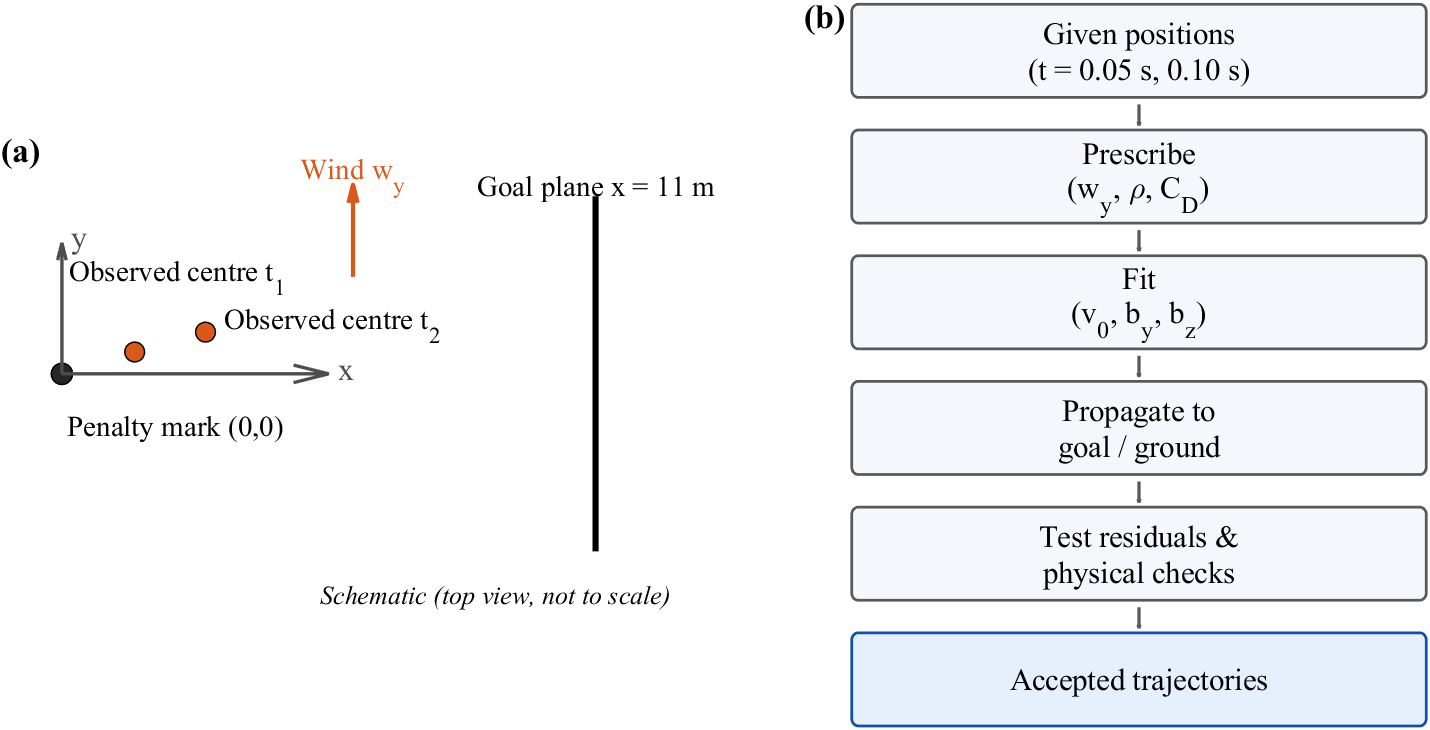
\includegraphics[width=\linewidth]{系统与反演流程.png}
\caption{Coordinate convention and the path from two observations to accepted trajectories. The left panel shows the horizontal geometry; the right panel shows listed environment values, fitted launch conditions, the allowed-error and physical checks, and the recorded terminal events.}
\label{fig:flow}
\end{figure}

\section{Physical model from kick to goal}
This section writes the force law used from the kick to the first terminal event.

The ball is a sphere of radius $R=0.11$ m and mass $m=0.43$ kg. The air is steady with lateral wind $\mathbf w=(0,w_y,0)$, constant density $\rho$, constant drag coefficient $C_D$, and a constant effective sideways coefficient $\mathbf b=(0,b_y,b_z)$. We use
\begin{equation}
\dot{\mathbf r}=\mathbf v,\qquad
\dot{\mathbf v}=\mathbf g-KC_D|\mathbf u|\mathbf u+\mathbf b\times\mathbf u,
\qquad \mathbf u=\mathbf v-\mathbf w,
\qquad K=\frac{\rho\pi R^2}{2m},
\label{eq:model}
\end{equation}
with $\mathbf g=(0,0,--9.81)$ m s$^{-2}$. The drag term is quadratic and opposes the motion relative to the air. The cross term is perpendicular to $\mathbf u$. The coefficient $\mathbf b$ has units s$^{-1}$ and combines rotation and lift efficiency; it is not the angular velocity, and we do not claim to recover the true spin. Setting $b_x=0$ removes a direction that the two positions constrain weakly. Constant coefficients, steady wind, no spin decay and no drag crisis are assumptions, not measurements; they are checked only as a model, not calibrated to this ball. The force form follows standard football aerodynamics~\cite{asai}.

\begin{table}[H]\centering
\caption{Symbols, units and roles. Listed environmental values are scenario inputs; launch conditions are inferred.}
\begin{tabular}{lll}\toprule
Symbol & Meaning & Unit or role\\\midrule
$\mathbf r,\mathbf v$ & Ball centre and velocity & m; m s$^{-1}$\\
$\mathbf u=\mathbf v-\mathbf w$ & Velocity relative to the air & m s$^{-1}$\\
$\mathbf w=(0,w_y,0)$ & Steady lateral wind & listed scenario input\\
$\rho$ & Air density & listed scenario input\\
$C_D$ & Drag coefficient & listed scenario input\\
$\mathbf b=(0,b_y,b_z)$ & Effective sideways coefficient & s$^{-1}$; inferred\\
$K$ & $\rho\pi R^2/(2m)$ & m$^{-1}$\\
$\epsilon$ & Allowed coordinate error & m\\
$C_\perp$ & Side-force coefficient $|\mathbf b\times\mathbf u|/(K|\mathbf u|^2)$ & dimensionless\\
$(t_g,y_g,z_g)$ & First crossing of $x=11$ m & s; m; m\\
\bottomrule\end{tabular}
\end{table}

The fixed mass and radius satisfy the IFAB ball specifications~\cite{ifab}. Density, wind and drag values are listed scenarios, not weather measurements. We do not model the goalkeeper, post collisions, deformation during contact, or flight after the first terminal event. The ball starts at the given centre with no vertical offset beyond the radius.

Over the roughly 0.4 s between kick and goal, the three terms can all change the path. Gravity bends the flight downward throughout. Drag grows with the square of the speed relative to the air, so a tailwind or headwind changes the deceleration as well as the direction of the relative flow. The sideways term grows with speed and with the fitted coefficients, and it bends the path without doing work, since $\mathbf b\times\mathbf u$ is perpendicular to $\mathbf u$. A model with gravity alone cannot connect the early positions to a late one, but the data do not measure the size of either aerodynamic term. That gap is why the paper treats the environmental values as listed inputs rather than known quantities.

\section{Finding parameters from the observations}
This section explains how the two positions become parameter choices.

For each listed triple $\eta=(w_y,\rho,C_D)$ we fit $q=(v_{0x},v_{0y},v_{0z},b_y,b_z)$ by bounded nonlinear least squares,
\begin{equation}
q^*(\eta)=\arg\min_{q\in\mathcal B}\sum_{i=1}^{2}
\|\mathbf r(t_i;q,\eta)-\mathbf r_i\|^2,
\label{eq:fit}
\end{equation}
using \texttt{lsqnonlin}~\cite{lsq} from two starting points. The trajectory in the fit is integrated with RK4 at the recorded step. A fit is checked on all six coordinates,
\begin{equation}
|r_j(t_i;q,\eta)-r_{ij}|\le\epsilon,
\qquad i=1,2,\quad j=x,y,z,
\label{eq:tol}
\end{equation}
at $\epsilon=2,5,10,20$ mm; 5 mm is the default. The allowed error is a stated scenario, not a measured camera accuracy.

The search uses 7 wind values on $[-8.000,8.000]$ m s$^{-1}$, 3 density values $\{1.100, 1.225, 1.350\}$ kg m$^{-3}$, and 10 drag values on $[0.15,0.60]$, giving 210 parameter choices. These values are example settings, not measured distributions. Only the listed parameter values are searched, and the ranges in the figures do not guarantee that all possible cases are included.

Before a fit is called accepted it also passes a physical screening. The launch must point forward and not downward, the initial speed must lie between 10 and 40 m s$^{-1}$, and along the sampled trajectory the side-force coefficient must satisfy $C_\perp\le0.50$. The ball must stay above the ground before the terminal event, and the event must be located within 2 s. An accepted fit must pass both the six-coordinate test and this screening; observation fit and physical screening are stored separately. The speed range and the 0.50 cap are conservative model screens, not universal limits for players or footballs. We do not force the crossing into the goal: a miss is a recorded outcome, and the goal is used only to describe where the ball goes.

Two further points explain why the result is a set rather than one shot. First, the fitting problem has more unknowns than the six coordinates. Changing the wind or the drag changes the air force, and a different launch velocity can make up for much of that change at the two observed times. The fit therefore finds different launch conditions for different listed environments, even though all of them look the same at $t=0.05$ and $t=0.10$ s. Second, the two observations constrain the early path only. A small difference in the fitted sideways coefficient can build into a larger sideways displacement over the remaining flight, because the force keeps acting after the last observation. The accepted set is the result of searching the listed values, not a proof that nothing outside the grid exists. Only the listed parameter values are searched, and the ranges in the figures do not guarantee that all possible cases are included.

\section{Results}
This section reports the current example, two accepted trajectories with different landings, and the screening figures.

For the current example the listed values are wind 8.0 m s$^{-1}$, density 1.225 kg m$^{-3}$, $C_D=0.350$, allowed error 5 mm, and maximum step 0.002 s. The fit gives
\begin{equation}
(v_{0x},v_{0y},v_{0z},b_y,b_z)=(30.4520, 9.4164, 6.9161, -0.0414, -0.5296),
\end{equation}
with the first three entries in m s$^{-1}$ and the last two in s$^{-1}$; the prescribed drag coefficient is $C_D=0.3500$. The largest coordinate residual is 0.915 mm, and the initial speed is 32.616 m s$^{-1}$. The ball first crosses $x=11$ m at
\begin{equation}
(y_g,z_g)=(2.6087,1.9598)\ \mathrm m,
\qquad t_g=0.4042\ \mathrm s.
\end{equation}
The recorded terminal status is \texttt{plane}, and the finite-radius opening check is yes. These numbers belong to this one parameter choice; they are not a unique answer, and no probability is implied.

Table~\ref{tab:tol} repeats the fit for every listed parameter choice at four allowed errors. Reading the 5 mm row: 86 of 210 choices are accepted, their crossings span the stated $y$ and $z$ ranges, and the Plane and Opening columns count arrivals and opening clearances. Ground-first outcomes are listed separately; they are not silently extrapolated below the ground.
\begin{table}[H]\centering
\caption{Allowed-error screening of the same parameter choices. Ranges are spreads over the sampled values, not uncertainty bounds.}
\label{tab:tol}
\begin{tabular}{rrrrrrr}\toprule
$\epsilon$ (mm) & Accepted & Plane & Opening & Ground & $y_g$ (m) & $z_g$ (m)\\\midrule
2 & 36/210 & 36 & 36 & 0 & $[2.5779,2.6227]$ & $[1.9578,1.9752]$ \\
5 & 86/210 & 86 & 86 & 0 & $[2.5384,2.6812]$ & $[1.9451,1.9867]$ \\
10 & 168/210 & 168 & 168 & 0 & $[2.4451,2.7562]$ & $[1.9183,2.0053]$ \\
20 & 210/210 & 210 & 210 & 0 & $[2.2802,2.8152]$ & $[1.8846,2.0125]$ \\
\bottomrule\end{tabular}\end{table}

The two displayed examples are taken from the accepted set at 5 mm; their positions in the MATLAB arrays are 13 and 47. Table~\ref{tab:pair} lists their values. Both reproduce the two positions within 5 mm, yet their crossings differ by 0.1477 m.

The two rows show the compensation directly. They use different wind and drag values, so the aerodynamic force differs, and the fitted launch speeds are not identical. Each shot also takes its own sideways coefficient to keep the same early positions. These differences also affect the rest of the flight and produce a gap at the goal plane. The gap is modest, and that is expected: these are steady force values fitted to the same two positions, and a more complex force law would not automatically make the answer more certain.
\begin{table}[H]\centering\small
\caption{Two accepted trajectories with different goal-plane crossings. Wind acts from the kick in both.}
\label{tab:pair}
\begin{tabular}{lrrrrrrrr}\toprule
 & $w_y$ & $\rho$ & $C_D$ & $|v_0|$ & Error (mm) & $y_g$ & $z_g$ & $t_g$\\\midrule
A & -8.0 & 1.225 & 0.2500 & 32.323 & 4.834 & 2.6812 & 1.9847 & 0.3906 \\
B & -5.3 & 1.225 & 0.4500 & 32.849 & 4.999 & 2.5389 & 1.9451 & 0.4099 \\
\bottomrule\end{tabular}
\par\smallskip\footnotesize Units: wind and speed in m s$^{-1}$; density in kg m$^{-3}$; plane coordinates in m; time in s.
\end{table}

Figure~\ref{fig:separation} explains why different goal points can fit the same observations. In the left panel, all six coordinate errors are within the allowed band for both examples. In the right panel, their late paths separate. Their launch conditions compensate for different aerodynamic forces during the measured interval, but this compensation does not keep the later positions identical.
\begin{figure}[H]\centering
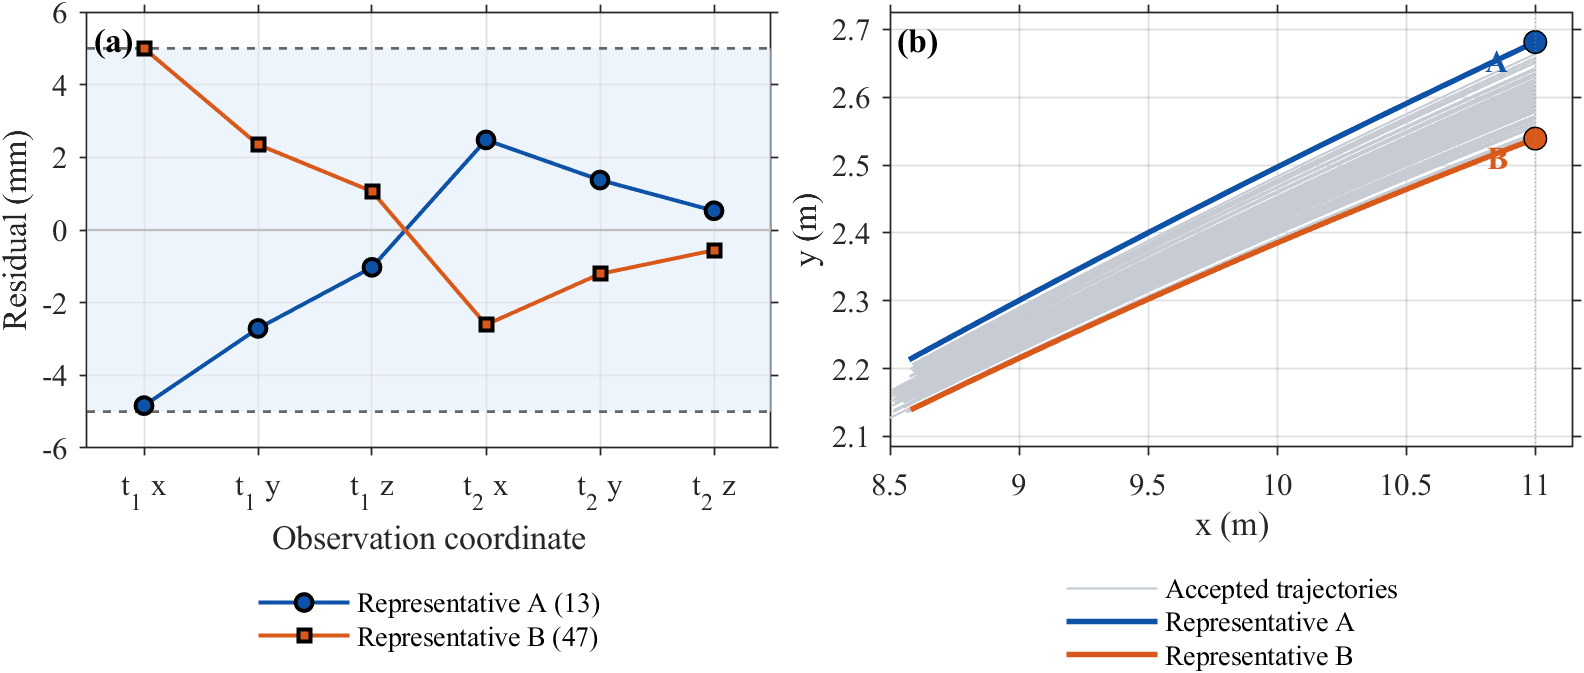
\includegraphics[width=.96\linewidth]{观测约束与轨迹分离.png}
\caption{The two accepted trajectories satisfy all six coordinate checks (left), but their late paths separate in the horizontal plane (right). The shaded band is the stated allowed error; displacements are shown at true scale.}
\label{fig:separation}
\end{figure}

Figure~\ref{fig:coupling} shows how the inputs and fitted quantities change together. A larger density--drag product generally requires a larger launch speed for these observations (left). The sideways coefficient changes with wind (middle). Increasing the allowed measurement error accepts more parameter choices (right).
\begin{figure}[H]\centering
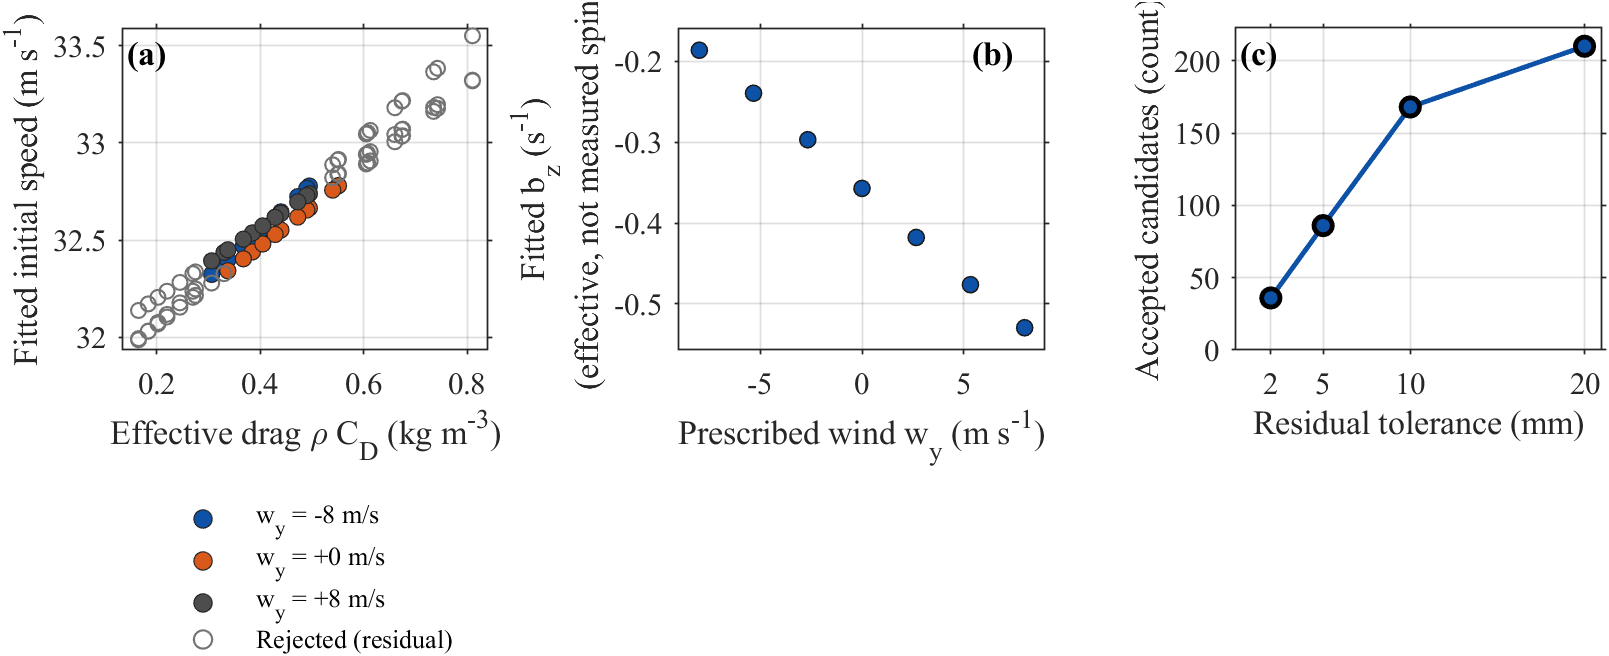
\includegraphics[width=\linewidth]{参数耦合与筛选敏感性.png}
\caption{Parameter coupling and screening: density--drag product against fitted launch speed for three wind slices (left); wind against the fitted $b_z$ for accepted trajectories (middle); accepted count against the allowed error (right). All counts refer to the listed parameter choices.}
\label{fig:coupling}
\end{figure}

The goal-plane view in Figure~\ref{fig:scatter} shows the range of crossing points from the accepted trajectories. Colour identifies the specified drag coefficient; the number of plotted points in a region carries no probability weight.
\begin{figure}[H]\centering
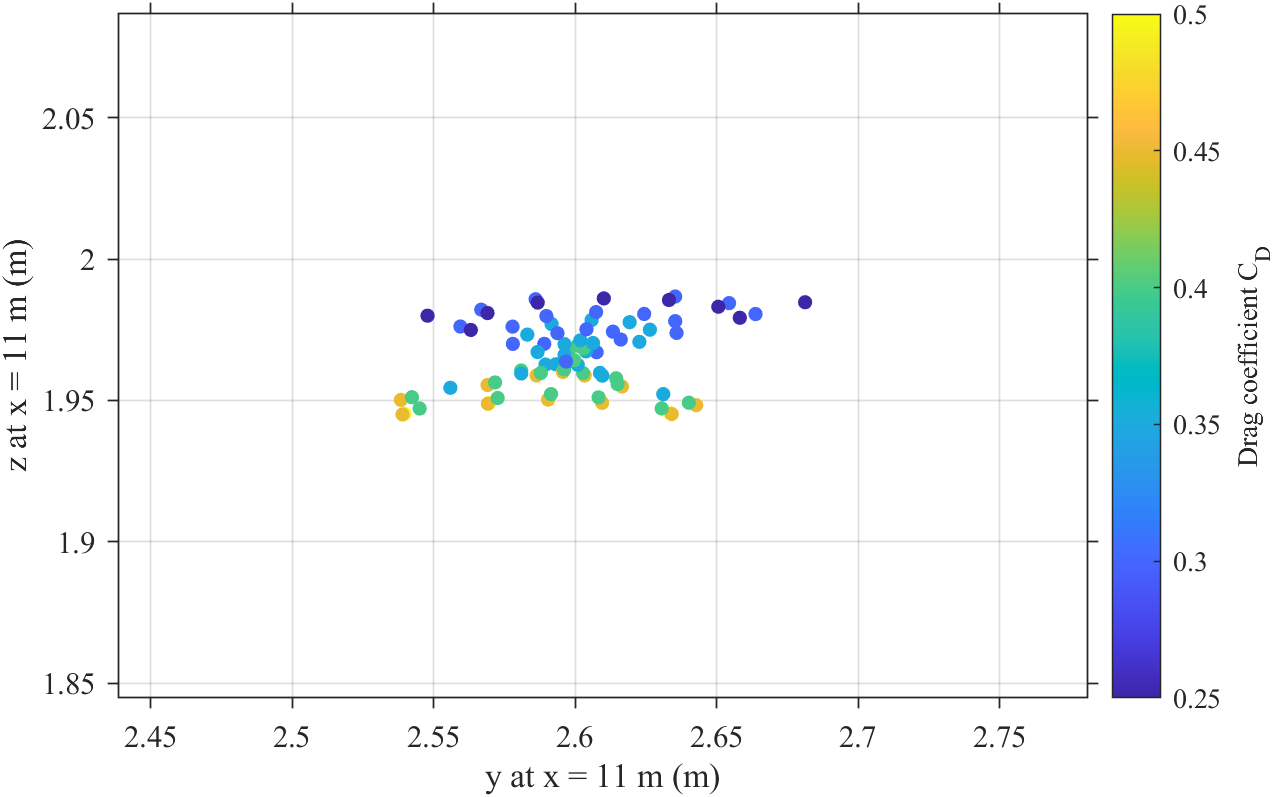
\includegraphics[width=.72\linewidth]{全程约束球门散点.png}
\caption{Goal-plane crossings of the accepted trajectories. Colour marks the listed drag coefficient. The spread is a property of the sampled parameter choices, not a probability distribution.}
\label{fig:scatter}
\end{figure}

A separate interactive view allows wind in $[-15,15]$ m s$^{-1}$, density in $[0.90,1.40]$ kg m$^{-3}$ and $C_D\in[0.08,0.80]$; this wider exploration is distinct from the paper grid and uses the same screening.

\section{Numerical checks and scope}
This section lists the checks made inside MATLAB and the limits of the result.

All calculations use the same equations and event definitions. The three step sizes differ only in the maximum step of the integration, so they measure numerical sensitivity rather than a new model. The work-energy check compares the change of mechanical energy with the work of drag and the sideways force,
\begin{equation}
\frac{d}{dt}\left(\frac12m|\mathbf v|^2+mgz\right)
=(\mathbf F_D+\mathbf F_M)\cdot\mathbf v.
\end{equation}
Event checks confirm that ground contact, the forward crossing of $x=11$ m and any time-out are located and recorded separately. The largest change in the goal-plane endpoint among the three step sizes is $6.66\times 10^{-15}$ m. The work-energy balance closes to $1.99\times 10^{-13}$ J. Checks with deliberately excessive launch speed and side force were rejected as intended.

These checks test the code and the internal balance. No independent measured full flight was available, so they do not confirm that this particular ball, field and camera obey the model. The reported crossings and ranges apply only to the listed parameter choices and the stated allowed error. They carry no probability and no guarantee outside the searched values. A wider allowed error accepts more trajectories, but it does not turn the sampled spread into a set that must contain the true landing point.

\section{Conclusion}
This section answers the problem.

From the two early positions, a single trajectory cannot be recovered when the wind and aerodynamic coefficients are unknown. For each listed environment we can still fit launch conditions that reproduce both positions, and those accepted trajectories cross the goal plane at different points. For the current example at wind 8.0 m s$^{-1}$ and density 1.225 kg m$^{-3}$, the centre crosses at $(2.6087,1.9598)$ m after 0.4042 s. Across the listed choices, 86 of 210 fits pass the 5 mm test, with crossings spanning $y\in[2.5384,2.6812]$ m and $z\in[1.9451,1.9867]$ m; two accepted trajectories differ by 0.1477 m. These ranges describe the sampled grid only and are not probabilities. More observation times, measured wind and a measured drag coefficient would narrow the answer.

\begingroup\small\raggedright
\begin{thebibliography}{9}
\bibitem{upc} University Physics Competition. 2026 contest, Problem B. \url{https://www.uphysicsc.com/2026contest.html}. Accessed 7 November 2026.
\bibitem{ifab} The IFAB. Laws of the Game, Law 2: The Ball. \url{https://www.theifab.com/laws/latest/the-ball/}. Accessed 7 November 2026.
\bibitem{asai} T. Asai, K. Seo, O. Kobayashi and R. Sakashita. Fundamental aerodynamics of the soccer ball. \emph{Sports Engineering} 10, 101--109 (2007). \url{https://doi.org/10.1007/BF02844207}.
\bibitem{ode} MathWorks. \texttt{ode45}: Solve nonstiff differential equations. \url{https://www.mathworks.com/help/matlab/ref/ode45.html}. Implementation run with MATLAB R2024a.
\bibitem{lsq} MathWorks. \texttt{lsqnonlin}: Solve nonlinear least-squares problems. \url{https://www.mathworks.com/help/optim/ug/lsqnonlin.html}.
\end{thebibliography}

\smallskip\small
\section*{Report on the use of AI}
AI tools assisted with code generation, numerical checks and manuscript drafting. Human team members must verify all adopted content and take responsibility for it.

\textbf{Team number and the complete AI records are still to be added; this is not a final submission.} The contest rules require the exact input and complete output of the AI tools used; that record must be appended and reviewed before submission.
\endgroup
\end{document}
